\documentclass[a4paper,11pt]{article}
\usepackage[utf8]{inputenc}
\usepackage[T1]{fontenc}
\usepackage[english]{babel}
\usepackage{times}
\usepackage{graphicx}
\textwidth=6in
\textheight=9.0in
\headheight=0in
\headsep=0in
\oddsidemargin=0in
\evensidemargin=0in
\title{SSM2164 SVF}
\author{Olivier Gillet -- \tt ol.gillet@gmail.com}
\date{}
\begin{document}

\maketitle

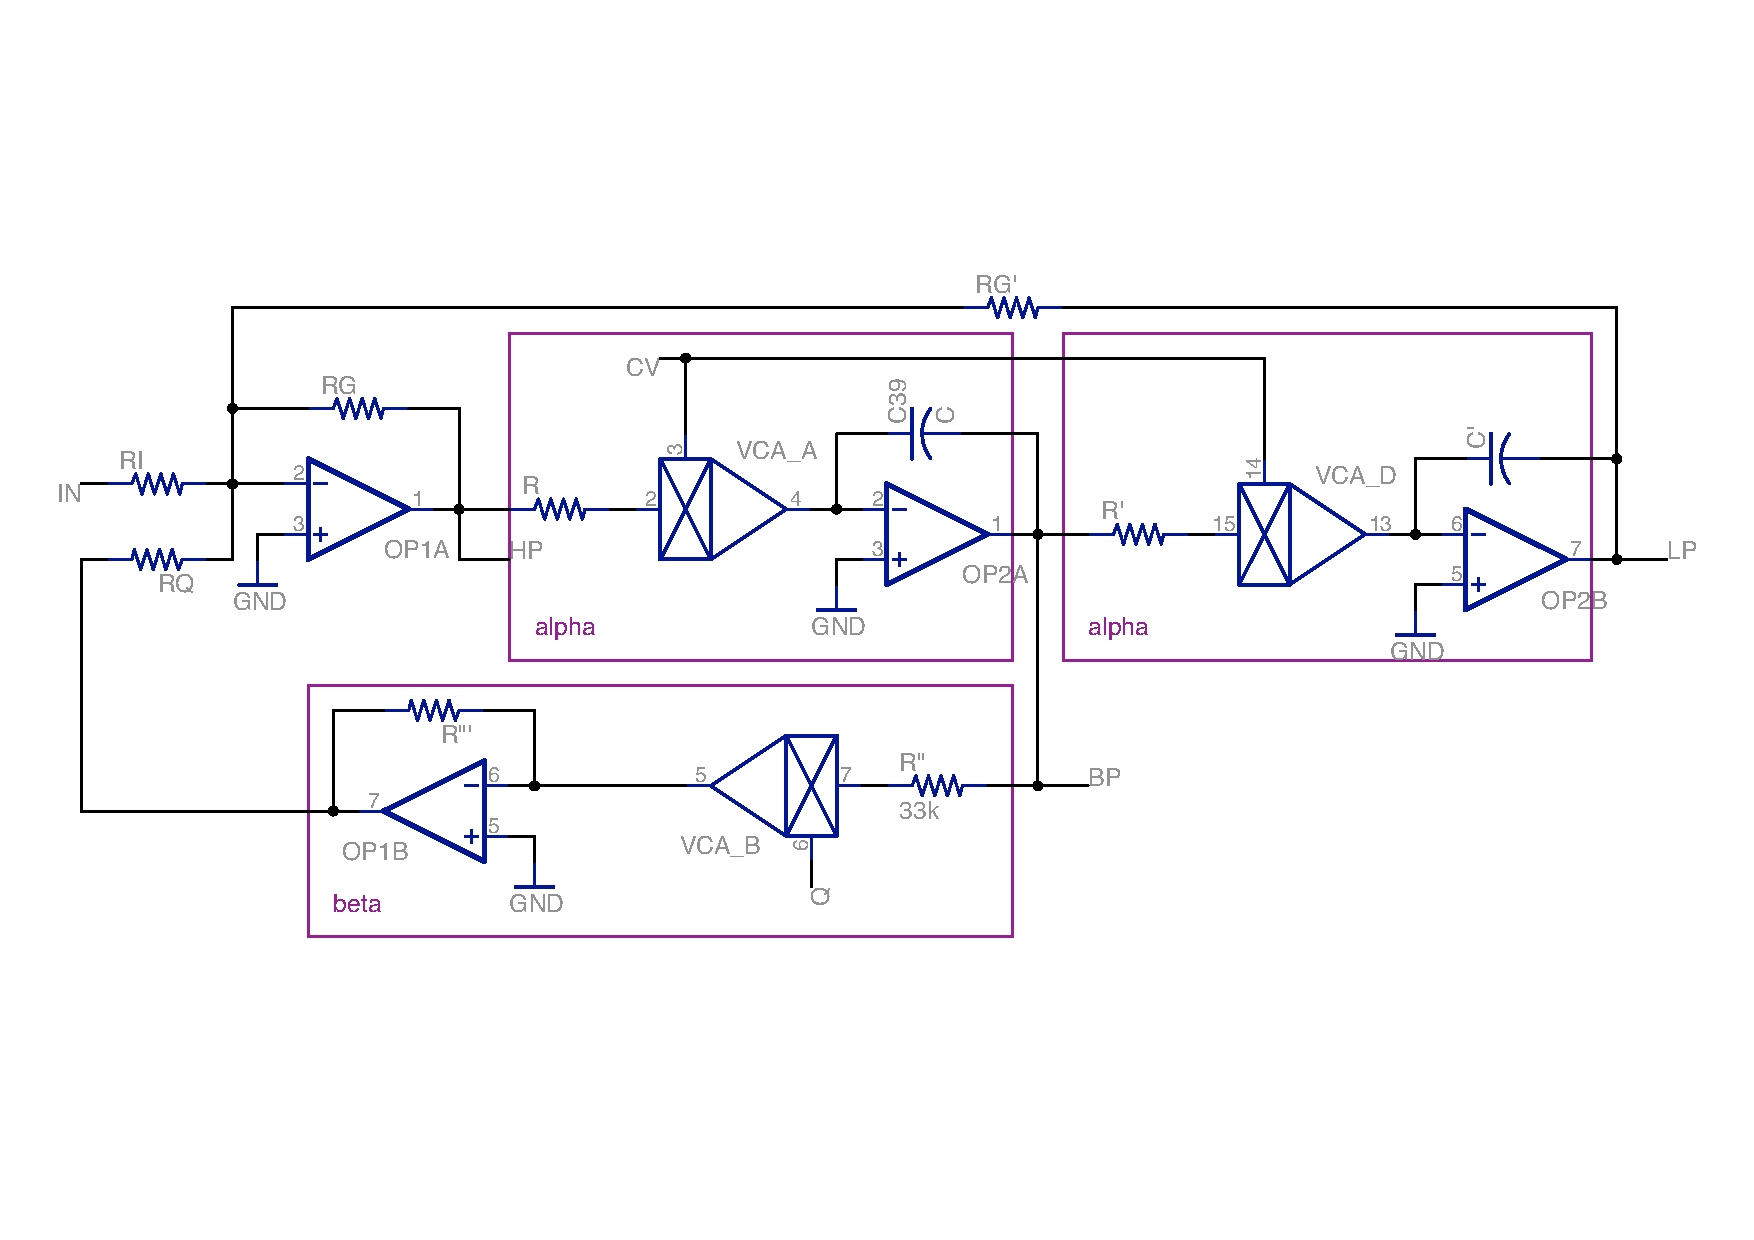
\includegraphics[width=\textwidth]{svf_schematics.pdf}


Notations:

$R_i$ is the value of the resistor through which the input signal is fed to the circuit.

$R_g$ is the value of the resistors through which the HP and LP output are fed back into the input.

$R$ is the value of the resistors through which input voltages are converted into currents at the input of the 2164s.

$R_b$ is a grounded resistor through which the current at the output of the Q gain cell is converted into a voltage.

$C$ is the value of the integrators' capacitors.

$v_{cv}$ is the cutoff frequency control voltage and $v_{q}$ is the Q control voltage.


The input voltage is $v_i(s)(s)$. $v_{lp}(s)$, $v_{hp}(s)$, $v_{bp}(s)$ are respectively the voltages at the low-pass, high-pass and band-pass nodes of this is the last candidate.  next esc will revert to uncompleted text. he circuit.

The transfer function of an integrator cell is noted $\alpha(s)$:

\begin{equation}
\alpha(s) = -\frac{1}{RCs} 10^{-\frac{3}{2} v_{cv}}
\end{equation}

Thus: $v_{bp}(s) = v_{hp}(s) \alpha(s)$, and $v_{lp}(s) = v_{hp}(s) \alpha^2(s)$.

The gain of the feedback circuit is noted $\beta$:

\begin{equation}
\beta = \frac{R_b}{R} 10^{-\frac{3}{2} v_{q}}
\end{equation}

Since the op-amp has a huge input impedance, we can assume the current flowing into $i^-$ is null:

\begin{equation}
\frac{v_i(s) - v^-(s)}{R_i} + \frac{v_{hp}(s) - v^-(s)}{R_g} + \frac{v_{lp}(s) - v^-(s)}{R_g} = i^- = 0
\end{equation}


The voltages at the inputs of the op-amp are equal, $v^-(s) = v^+(s) = \alpha(s) \beta v_{hp}(s)$, hence:

\begin{eqnarray}
\frac{v_i(s) - \alpha(s) \beta v_{hp}(s)}{R_i} + \frac{v_{hp}(s) - \alpha(s) \beta v_{hp}(s)}{R_g} + \frac{v_{lp}(s) - \alpha(s) \beta v_{hp}(s)}{R_g} &=& 0 \\
\frac{v_i(s) - \alpha(s) \beta v_{hp}(s)}{R_i} + \frac{v_{hp}(s) - \alpha(s) \beta v_{hp}(s)}{R_g} + \frac{\alpha^2(s) v_{hp}(s) - \alpha(s) \beta v_{hp}(s)}{R_g} &=& 0
\end{eqnarray}

The transfer function for the HP mode is:

\begin{eqnarray}
H_{hp}(s) &=& \frac{v_{hp}(s)}{v_i(s)} \\
 &=& \frac{-1 / R_i}{\frac{-\alpha(s) \beta}{R_i} + \frac{1}{R_g} - 2 \frac{\alpha(s) \beta}{R_g} + \frac{\alpha^2(s)}{R_g}} \\
 &=& \frac{-1 / R_i}{\frac{1}{R_g} - \alpha(s) \beta \left(\frac{1}{R_i} + 2 \frac{1}{R_g}\right) + \frac{\alpha^2(s)}{R_g}} \\
 &=& \frac{-R_g / R_i}{1 - \alpha(s) \beta \left(\frac{R_g}{R_i} + 2\right) + \alpha^2(s)} \\
 &=& \frac{-G}{1 - \alpha(s) \beta \left(G + 2\right) + \alpha^2(s)}
\end{eqnarray}

$G = \frac{R_g}{R_i}$ is the absolute value of the pass-band gain.

The transfer function for the LP mode is:

\begin{eqnarray}
H_{lp}(s) &=& \frac{v_{lp}(s)}{v_i(s)} \\
 &=& \frac{v_{hp}(s)}{v_i(s)} \alpha^2(s) \\
 &=& \frac{-G}{\frac{1}{\alpha^2(s)} - \frac{\beta}{\alpha(s)} (G + 2) + 1} \\
 &=& \frac{-G}{\frac{s^2}{{\left(\frac{1}{RC} 10 ^ {-\frac{3}{2} v_{cv}}\right)}^2} + \frac{s}{{\left(\frac{1}{RC} 10 ^ {-\frac{3}{2} v_{cv}}\right)}} \beta (G + 2) + 1}
\end{eqnarray}

This gives the following filter characteristics:

\begin{itemize}
\item Pass-band gain, $-G = -\frac{R_g}{R_i}$
\item Cutoff frequency, $f = \frac{1}{2 \pi R C} 10 ^ {-\frac{3}{2} v_{cv}}$
\item Q factor, $Q = \frac{1}{G + 2} \frac{1}{\beta} = \frac{1}{G + 2} \frac{R}{R_b} 10^{\frac{3}{2} v_{q}} $

\end{itemize}

\end{document}
